\section{Regime-dependent principle of hierarchical memory orchestration}
\label{sec:regime}

Hierarchical memory coordination is often treated as a smooth trade-off: as long as transfers are overlapped and data are cached, additional orchestration should yield monotonic (if diminishing) gains. We argue that this intuition is structurally incomplete. In multi-tier systems, \emph{dimensionless control parameters} that capture (i) residency of the active working set in fast memory and (ii) sustained transfer pressure on the slowest tier induce \emph{phase-like} behavior. Once a critical threshold is crossed, the dominant latency contributor changes abruptly, and coordination/synchronization overheads that were previously amortized become exposed. This is why the same offloading or swapping strategy can appear highly effective in one setting and predictably fail in another.

This section establishes the core principle of this work: hierarchical memory orchestration in AI inference systems is inherently regime-dependent, exhibiting qualitatively distinct operational modes rather than a continuously optimizable spectrum.


\subsection{Hierarchical memory systems beyond continuous optimization}
Hierarchical memory systems are a defining feature of modern AI inference platforms. Accelerator memory provides high bandwidth and low latency but is severely capacity-limited, while host memory and secondary storage offer progressively larger capacity at the cost of increasing access latency and lower bandwidth. As model sizes and intermediate working sets grow beyond fast-memory capacity, inference performance inevitably depends on coordination across these tiers.

A dominant assumption in much of the existing literature is that hierarchical coordination is \emph{continuously optimizable}. Under this assumption, performance degradation due to limited fast memory can be progressively mitigated through increasingly sophisticated orchestration mechanisms---such as caching, offloading, swapping, or overlapping computation with data transfer. From this perspective, additional coordination is expected to yield diminishing but monotonic improvements.

Empirical behavior in large-scale inference systems, however, frequently contradicts this assumption. Systems often exhibit abrupt performance degradation, instability, or even performance inversion when memory pressure, transfer traffic, or synchronization overhead exceeds certain thresholds. These observations indicate that hierarchical memory orchestration is not governed by smooth trade-offs but by structural constraints that give rise to qualitatively different modes of operation.

Here, we argue that hierarchical memory orchestration is fundamentally \emph{regime-dependent}. Rather than forming a single continuum of optimizable configurations, multi-tier memory systems operate within distinct regimes defined by intrinsic relationships among memory capacity, bandwidth, and coordination overhead. Within each regime, different latency components dominate end-to-end performance, and optimization strategies that are effective in one regime may fail predictably in another.

\subsection{Operational regimes in multi-tier memory systems}
We identify three primary operational regimes that characterize inference behavior under hierarchical memory systems. These regimes are not tied to specific hardware platforms or software implementations; instead, they emerge whenever working sets exceed fast-memory capacity and execution relies on cross-tier data movement.

\textbf{Capacity-limited regime.} In the capacity-limited regime, fast memory is insufficient to hold the working set required for efficient execution. Data reuse is therefore constrained, and execution incurs frequent eviction and reloading regardless of orchestration strategy. In this regime, locality effects dominate performance: even minimal coordination overhead cannot compensate for the lack of effective fast-memory residency.

\textbf{Coordination-dominated regime.} In the coordination-dominated regime, fast and intermediate memory tiers together can absorb most of the working set, but performance is sensitive to how data movement and synchronization are orchestrated. Here, computation, memory locality, transfer overhead, and synchronization costs are of comparable magnitude. In this regime, orchestration can reshape end-to-end behavior by reducing redundant movement, improving locality, and overlapping computation with transfer.

\textbf{I/O-limited regime.} In the I/O-limited regime, cross-tier data transfer approaches or exceeds the sustained bandwidth of the slowest memory tier. Physical transfer constraints dominate execution, and coordination overhead becomes additive rather than compensatory. Once transfer demand saturates available bandwidth, latency scales with data movement, and additional coordination increases overhead without improving throughput.

\begin{figure}[t]
\centering
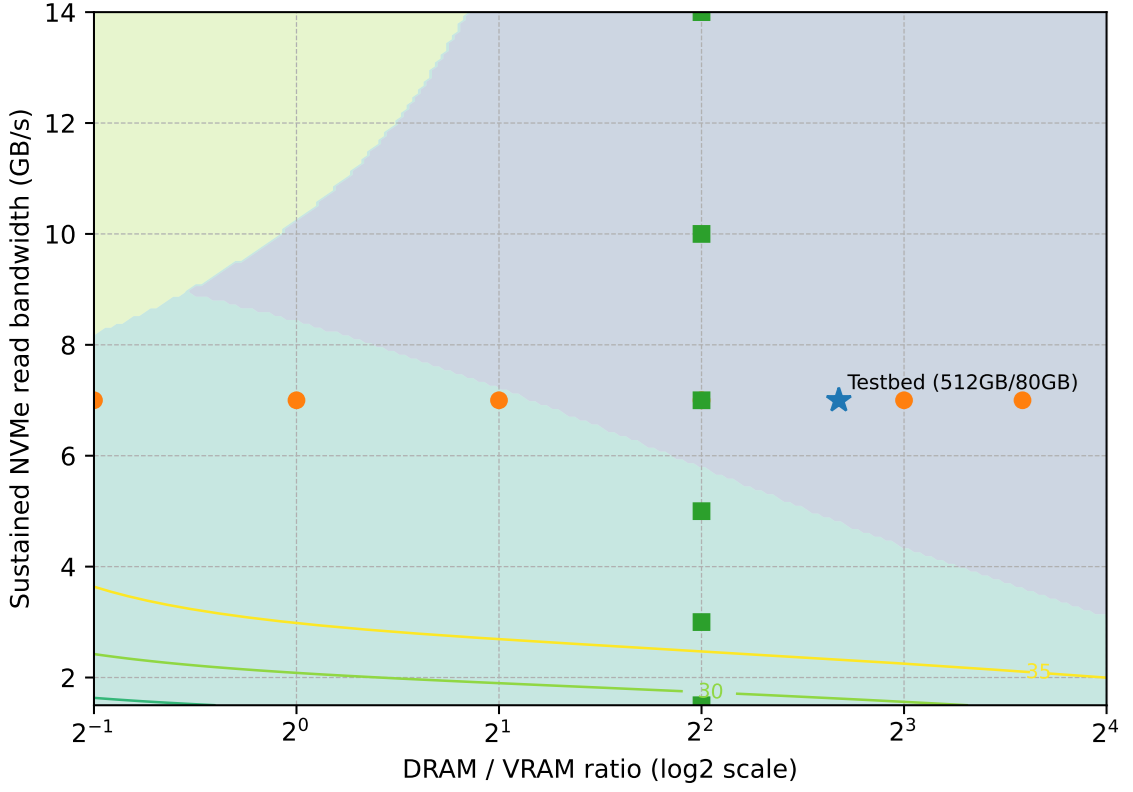
\includegraphics[width=0.95\linewidth]{figures/orion_regime_map.png}
\caption{\textbf{Regime-dependent behavior of hierarchical memory systems.} Dashed lines indicate analytically identified regime boundaries, separating capacity-limited, coordination-dominated, and I/O-limited regions. Shaded regions highlight empirically observed failure zones, including abrupt latency spikes and performance collapse beyond regime boundaries.
}
\label{fig:regime_map}
\end{figure}

Figure~\ref{fig:regime_map} illustrates the regime map and the boundaries separating capacity-limited, coordination-dominated, and I/O-limited behavior.

\subsection{Regime transitions as intrinsic system behavior}
Transitions between operational regimes are characterized by abrupt shifts in the dominant contributors to inference latency. As a system crosses a regime boundary---for example, due to changes in model size, batch size, memory capacity, or available storage bandwidth---the primary bottleneck can change discontinuously, shifting from locality-driven memory effects to coordination overhead, or from coordination to cross-tier data transfer.

This behavior directly challenges the assumption that hierarchical memory orchestration is continuously optimizable. Within coordination-dominated regimes, orchestration mechanisms can effectively reduce end-to-end latency by redistributing costs among computation, memory access, data movement, and synchronization. However, once a system enters a capacity-limited or I/O-limited regime, these same mechanisms lose their effectiveness: coordination overhead that was previously amortized becomes exposed, leading to predictable performance degradation rather than incremental improvement.

Crucially, such regime transitions are intrinsic properties of hierarchical memory systems rather than artifacts of specific implementations or optimization strategies. They arise from fundamental physical constraints on memory capacity and sustained transfer bandwidth, combined with unavoidable synchronization and coordination costs. As a result, regime transitions persist across workloads, model architectures, and hardware platforms, even as absolute performance levels vary.

This regime-based perspective reframes hierarchical memory orchestration as a problem of operating within feasible regimes defined by structural constraints, rather than endlessly tuning coordination mechanisms along a single continuous spectrum. The following section formalizes this intuition using a minimal analytical transfer model that makes regime boundaries explicit.


\FloatBarrier